\section*{Appendix}

\subsubsection{Questionnaires} % (fold)
\label{ssub:questionnaires}

\begin{figure}[H]
  \begin{center}
    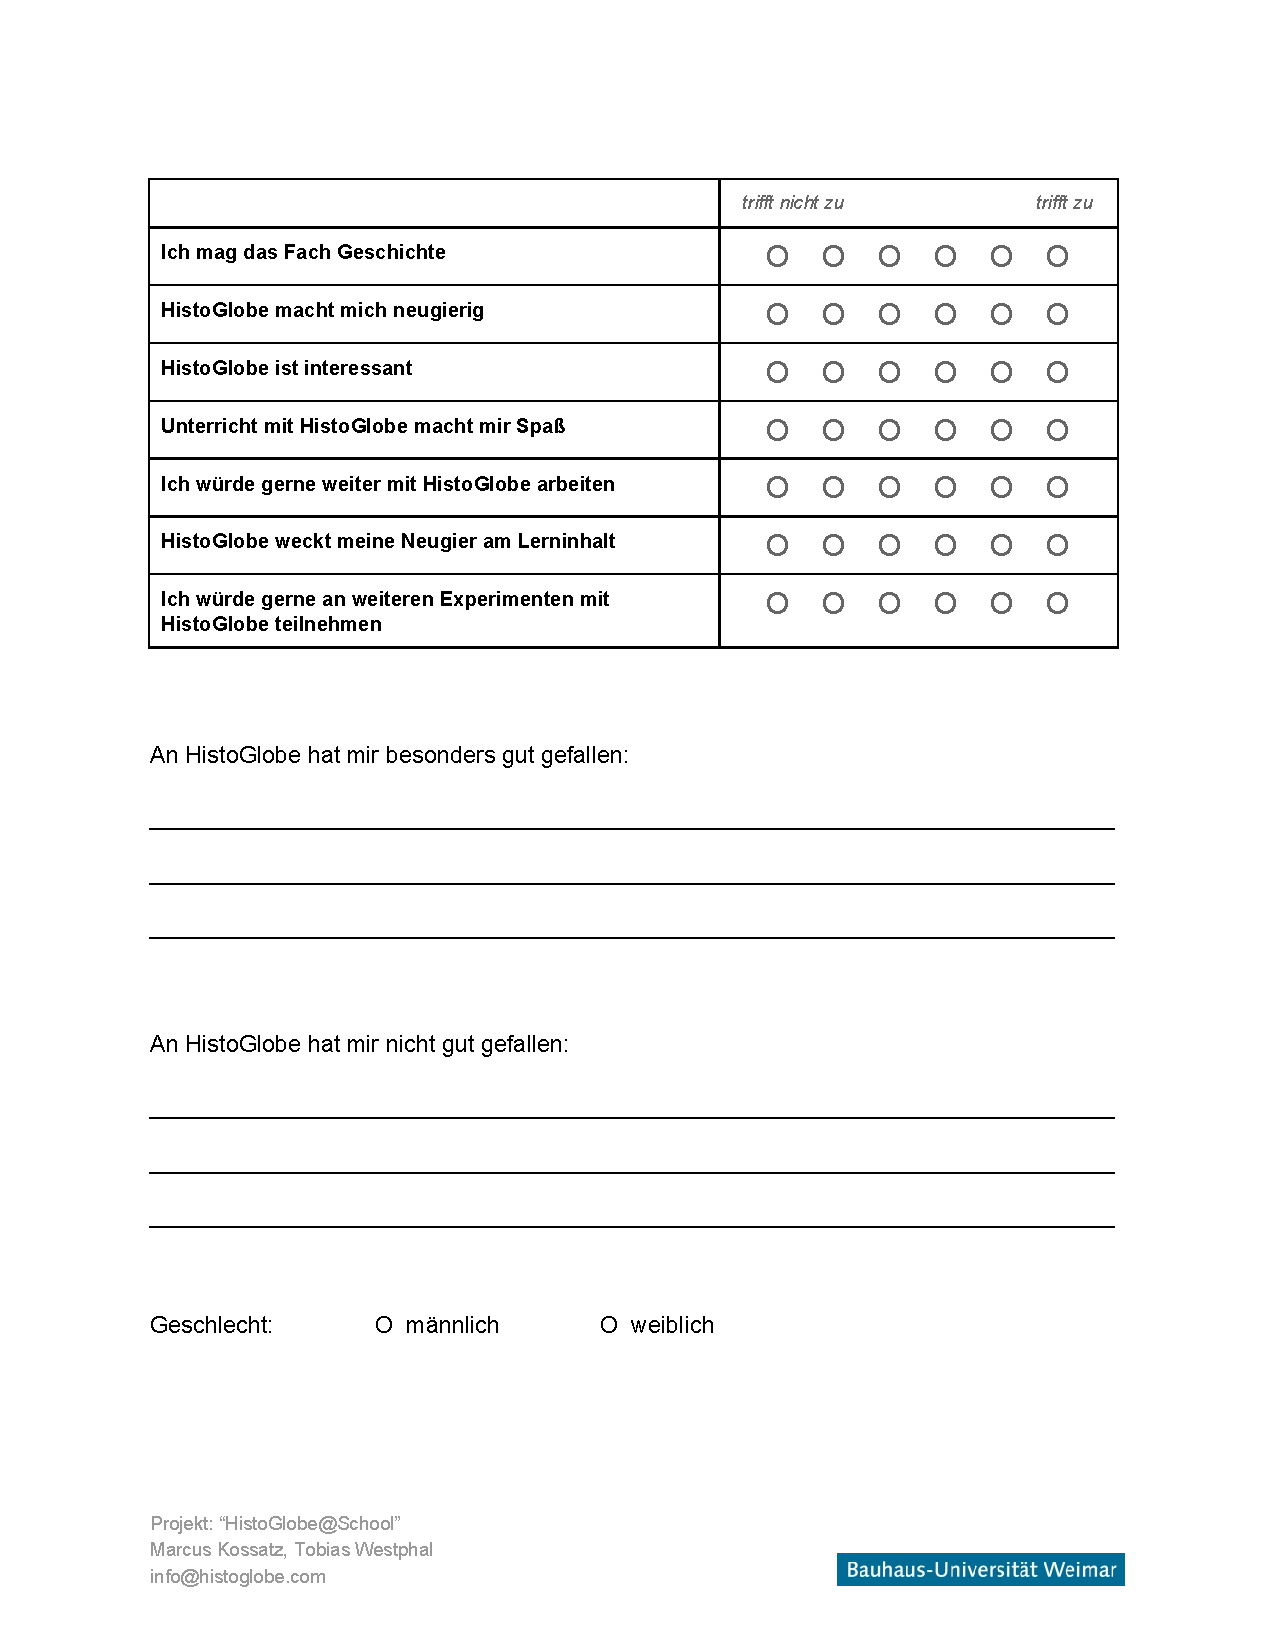
\includegraphics[width=1.0\textwidth]{graphics/questionnaire.pdf}
  \end{center}
  \caption{The questionnaire for the students}
  \label{fig:questionnaire}
\end{figure}

% subsubsection questionnaires (end)

\subsection{Work division}

\subsubsection{Marcus} % (fold)
\label{ssub:marcus}

\begin{itemize}
  \item Organization
  \begin{itemize}
    \item Administration of the Masterplan (Figure \ref{fig:masterplan})
    \item Responsibility for GIT branching and merging
    \item Email communication with the team members, the teachers, and project supervisors
  \end{itemize}
  \item Research Presentation
  \begin{itemize}
    \item The Browser (history, sandbox, components, flow, JS memory management)
  \end{itemize}
  \item User Centered Design:
  \begin{itemize}
    \item Throughout the project -- every two weeks
    \begin{itemize}
      \item Meeting the teacher in Jena
      \item Testing the current concept and implemented functionality
      \item Deriving new requirements
      \item Update the concept
    \end{itemize}
    \item End of the project: planning, designing, conducting and analyzing two field studies
  \end{itemize}
  \item Implementation
  \begin{itemize}
    \item Data Acquisition: Hivents
    \item Data Acquisition: Historical Countries
    \item Data Acquisition: Historical Changes
    \item Data Acquisition: Historical Topics and Theme Alliances in Bipolar World
    \item Preprocessing: areas, labels, transitions and changes
    \item Time-dependent areas on the map (geometry, labels, animated transitions)
    \item Theme- and time-dependent styling of the areas on the map
  \end{itemize}
  \item Final Documentation
  \begin{itemize}
    \item \ref{sec:user_centered_design} \nameref{sec:user_centered_design}
    \item \ref{sec:user_interface_elements} \nameref{sec:user_interface_elements}
    \item \ref{sub:map} \nameref{sub:map}
    \item \ref{sec:field_study} \nameref{sec:field_study}
  \end{itemize}
\end{itemize}

% subsubsection marcus (end)

\subsubsection{Max Weber} % (fold)
\label{ssub:max_weber}

\begin{itemize}
  \item
  \item
  \item
  \item
  \item
  \item
\end{itemize}

% subsubsection max_weber (end)

\subsubsection{Chris Hornischer} % (fold)
\label{ssub:chris_hornischer}

\begin{itemize}
  \item Research Presentation
  \begin{itemize}
    \item JavaScript Performance
  \end{itemize}
  \item Implementation
  \begin{itemize}
    \item Search Bar module (together with Max Weber)
    \item Hivent Box: positioning
    \item Hivent Box: drag and drop
    \item Hivent Box: content generation
    \item Hivent Box: big version
    \item Hivent Box: multimedia slide
  \end{itemize}
  \item Final Documentation
  \begin{itemize}
    \item \ref{sub:search_bar} \nameref{sub:search_bar}
    \item \ref{sub:hivent_boxes} \nameref{sub:hivent_boxes}
    \item \ref{sub:control_buttons} \nameref{sub:control_buttons}
    \item \ref{sec:conclusion} \nameref{sec:conclusion}
  \end{itemize}
\end{itemize}

% subsubsection chris_hornischer (end)

\subsubsection{Sebastian Koepsel} % (fold)
\label{ssub:sebastian_koepsel}

\begin{itemize}
  \item
  \item
  \item
  \item
  \item
  \item
\end{itemize}

% subsubsection sebastian_koepsel (end)

\subsubsection{Masterplan} % (fold)
\label{ssub:masterplan}

\begin{figure}[H]
  \begin{center}
    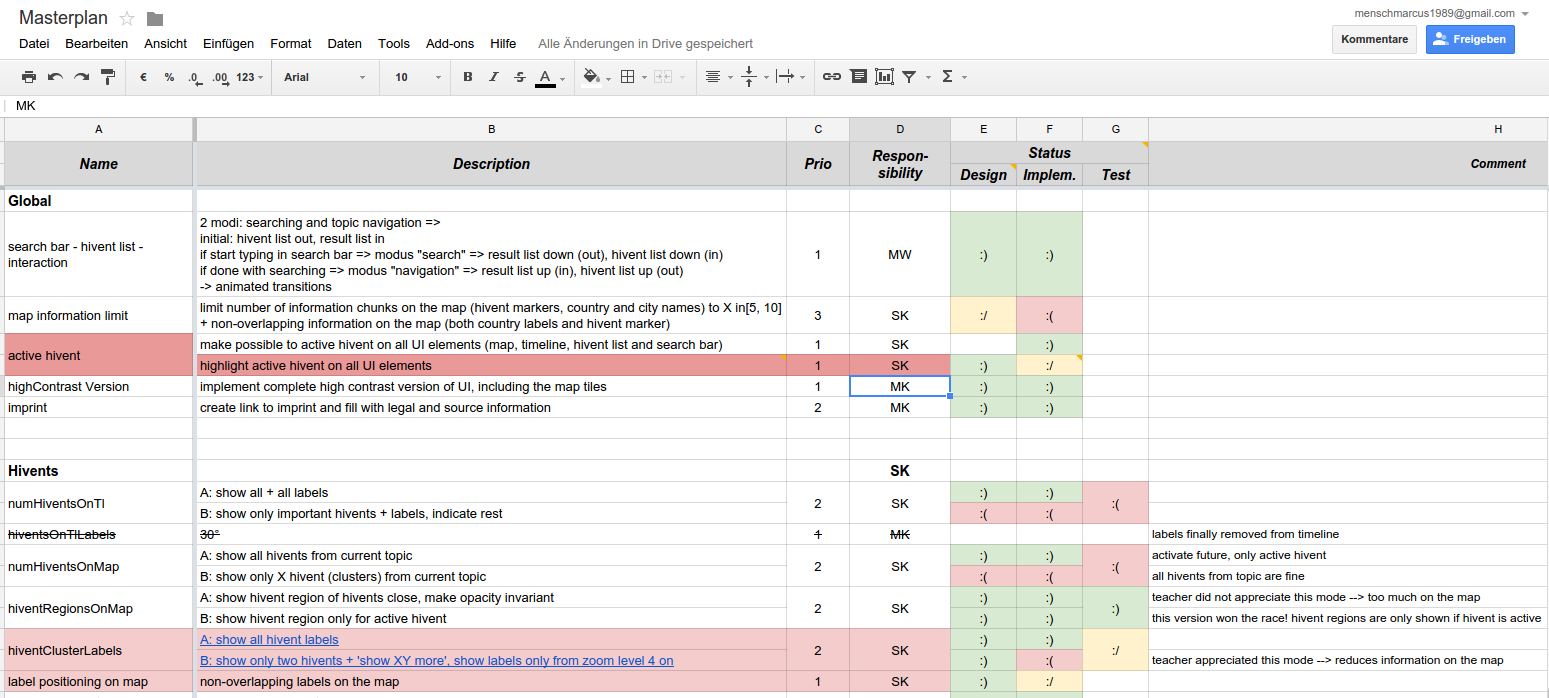
\includegraphics[width=0.9\textwidth]{graphics/Masterplan.png}
  \end{center}
  \caption{Extraction from the Masterplan of the project}
  \label{fig:masterplan}
\end{figure}

% subsubsection masterplan (end)

\subsubsection{GIT } % (fold)
\label{ssub:git_}

\begin{figure}[H]
  \begin{center}
    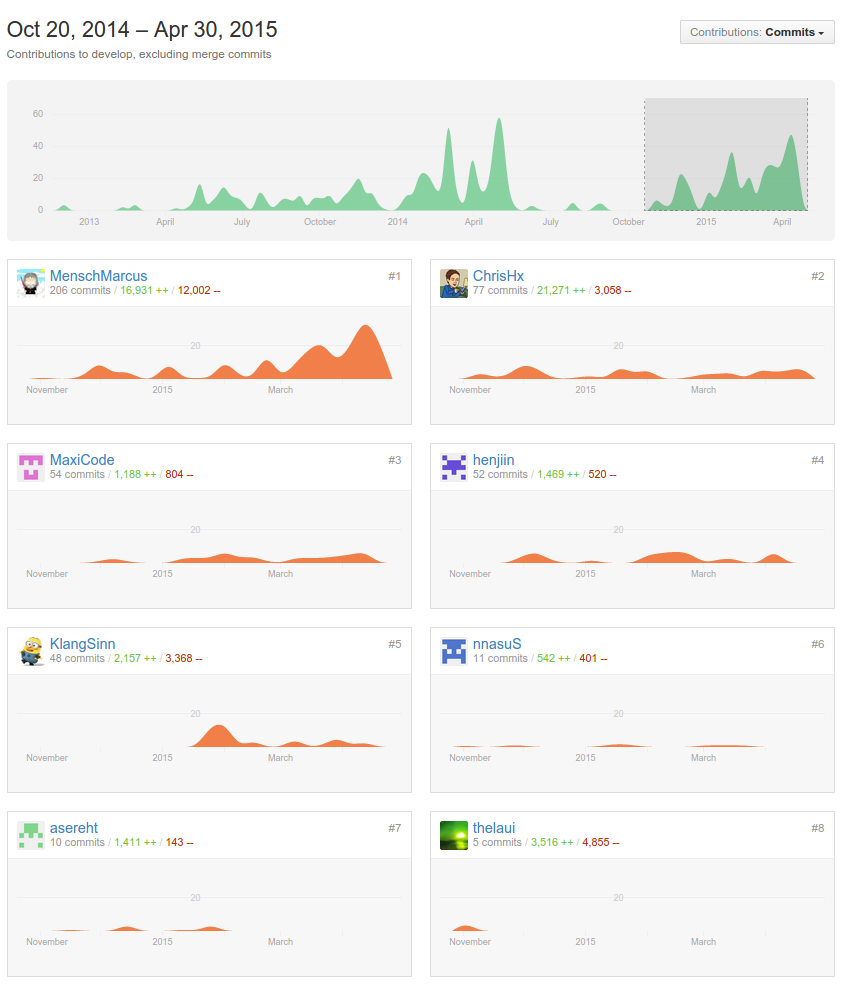
\includegraphics[width=1\textwidth]{graphics/git.png}
  \end{center}
  \caption{Collaborators of the git project HistoGlobeAtSchool}
  \label{fig:git}
\end{figure}

\begin{center}
\begin{small}
  \texttt{MenschMarcus}: Marcus Kossatz, \texttt{ChrisHx}: Chris Hornischer, \\
  \texttt{MaxiCode}: Max Weber, \texttt{henjiin}: Sebastian Koepsel
\end{small}
\end{center}

% subsubsection git_ (end)
